
\documentclass[journal,onecolumn]{IEEEtran}
\usepackage{float}
	\usepackage[spanish,es-tabla]{babel}
	% correct bad hyphenation here
	\hyphenation{op-tical net-works semi-conduc-tor}
	\usepackage{csquotes} % One of the things you learn about LaTeX is at some level, it's like magic. The references weren't printing as they should without this line, and the guy who wrote the package included it,
		\usepackage{graphicx}
	\graphicspath{ {./imgs/} }
	\begin{document}
		
	
	
		\title{Caracterización de personajes y generación de libretos para cortometrajes usando LLMs}
	
		
		\author{William Salamanca,~\IEEEmembership{Ingenieria de Sistemas y Computación,~UPTC}\\
			Yasser Cristancho,~\IEEEmembership{Ingenieria de Sistemas y Computación,~UPTC}}% <-this % stops a space
		
	\maketitle
	
	
	%\begin{abstract}
		%The abstract goes here.
	%\end{abstract}
	
	
	
	% Note that keywords are not normally used for peerreview papers.
	\begin{IEEEkeywords}
		LLM, AI, PLN, Fine Tunning, Transformer
	\end{IEEEkeywords}
	
	\IEEEpeerreviewmaketitle
	
	
	
	\section{Introducción}

	\IEEEPARstart{E}n la industria cinematográfica también se ha evidenciado el crecimiento de la revolución digital, aportando avances tecnológicos en la generación de productos visuales. Sin embargo, uno de los aspectos más fundamentales como la creación de personajes y la escritura de libretos sigue siendo muy manual.
	
	Dentro del entorno cinematográfico, los cortometrajes permiten brindar una visualización de entretenimiento en corto tiempo a los espectadores para dejar un mensaje o transmitir emociones a partir de una historia. Para la creación de un cortometraje, la caracterización y la creación de un libreto son fundamentales para construir historias memorables y cautivadoras. Los personajes bien definidos con sus características únicas son la base de cualquier narración. Por otro lado, la creación de libretos requiere tener un amplio dominio en escritura y el arte de generar historias de manera atractiva, lo que puede llevar mucho tiempo.
	
	Los Modelos de Lenguaje Largos o Extensos, de su traducción en sus siglas en inglés LLM (Language Large Models), han permitido evidenciar la capacidad potencial de generar texto o contenido para diferentes tareas \cite{reference1}. Contemplando lo anterior, en este proyecto se propone desarrollar un sistema que pueda analizar la narrativa del fragmento de un libro con el fin de explorar la aplicación de LLM para la identificación de personajes con sus características detalladas y la generación de libretos dependiendo del contexto que se ingrese en términos de ubicación, época, entre otros.

	
	\section{Planteamiento del problema}
	
	
	En la etapa de preproducción de una obra, guion o cortometraje, la creación de personajes detallados y bien definidos es fundamental para construir una historia cautivadora y convincente. Sin embargo, este proceso suele ser laborioso y requerir una amplia investigación y esfuerzo creativo por parte de los guionistas y directores. Mediante la implementación de un modelo LLM especializado en caracterización de personajes, se busca automatizar y agilizar esta tarea, permitiendo la generación de descripciones detalladas y coherentes de personajes a partir de un fragmento de una narrativa corta.
	
	Por otra parte, la escritura del libreto es una etapa crucial en la producción cinematográfica de cortometrajes. Requiere habilidades narrativas, conocimiento del formato de guiones y una gran inversión de tiempo. Al utilizar un modelo LLM entrenado específicamente para la generación de libretos, se pretende agilizar este proceso, brindando a los guionistas y directores una herramienta poderosa que les permita obtener borradores iniciales de libretos a partir de una idea.
	
	El objetivo principal de este proyecto es desarrollar una solución innovadora que aproveche la potencia de los modelos de lenguaje grandes (LLM) para facilitar y agilizar dos tareas clave en la producción de cortometrajes: la caracterización de personajes y la generación de libretos. Estos modelos serán entrenados con conjuntos de datos específicos y relevantes para cada tarea, utilizando técnicas de aprendizaje supervisado, buscando ahorrar tiempo y recursos.
	\section{Marco Conceptual}
	\subsection{Procesamiento de Leguaje Natural}
	El PLN es un campo de la informática que se ocupa de la interacción entre las computadoras y el lenguaje humano. Se centra en el desarrollo de métodos para que las computadoras puedan comprender, procesar y generar lenguaje natural.
	\subsection{Inteligencia Artificial}
	Es una rama de la informática que se ocupa del desarrollo de sistemas capaces de realizar tareas que normalmente requieren inteligencia humana, como el aprendizaje, la percepción, el razonamiento y la resolución de problemas. 
	\subsection{LLM}
	Los Modelos de Lenguaje Grandes (LLM, por sus siglas en inglés) son modelos de lenguaje entrenados en grandes cantidades de datos de texto, con millones o miles de millones de parámetros, lo que les permite capturar y representar relaciones complejas y sutilezas en el lenguaje natural
	\subsection{Transformer}
	El Transformer es una arquitectura de redes neuronales que se ha convertido en el estándar de facto para tareas de procesamiento de lenguaje natural, como la traducción automática, el resumen de texto y la generación de texto
	\subsection{Fine Tunning}
	El Fine-Tuning, o ajuste fino, es una técnica utilizada en el aprendizaje de transferencia, donde un modelo preentrenado se ajusta aún más en un conjunto de datos específico de la tarea objetivo, lo que permite adaptar el modelo a un dominio o tarea particular
	\section{Metodología}
	\subsection{Explorar LLMs}
	Se necesita tener una vista general de la variedad de LLMs que se encuentran actualmente implementados y desplegados.
	\subsection{Explorar documentación de los LLMs}
	Identificar aspectos relacionados a los requerimientos básicos y/o necesarios de los LLMs para poder hacer finetune de estos. Requerimientos de software y hardware, así como posibles comparativas que indiquen su desempeño en tareas de NPL, específicamente en las de identificar, caracterizar y clasificar personajes de libros. Además de la generación de libretos para cortometrajes a partir de personajes identificados, caracterizados y clasificados, y de un contexto histórico en el que se desarrolla el libreto.
	\subsection{Explorar fuentes de datos}
	Para el proceso de finetune de un LLM seleccionado se necesita tener varias fuentes de datos que en un principio nos provean de una descripción de las características de los personajes que se encuentran en este. Adicionalmente a lo anterior, se necesitan datos sobre contextos historicos con el fin de tener un contexto en el que se desarrolla el libreto para el cortometraje.
	\subsection{Comparativa inicial entre LLMs seleccionados}
	\begin{itemize}
		\item Capacidad de los modelos para realizar las tareas de identificación, caracterización y clasificación de personajes, además de la generación de libretos con base a lo anterior y un contexto historio dado.
		\item Tamaños y complejidades asociados a los modelos.
		\item Disponibilidad y acceso.
		\item Requerimientos de hardware.
	\end{itemize}
	\subsection{Comparativa mediante ejercicios entre LLMs seleccionados}
	Partiendo de las mismas entradas y con las mismas condiciones de hardware, identificar el que tenga mejor rendimiento en términos de tiempo pero, teniendo en cuenta la calidad de la salida.
	\subsection{Herramientas}
	\begin{itemize}
		\item Lenguaje de programación: Python.
		\item Bibliotecas: Hugging Face Transformers.
		\item Modelos Preentrenados: T5.
		\item Entorno: GoogleColab.
		\item Control de Versiones: Git y GitHub.
		\item Pypdf: Librería para extraer texto de PDFs
	\end{itemize}
	
	\section{Exploración de herramientas seleccionadas}
	\begin{figure}[H]
		\centering
		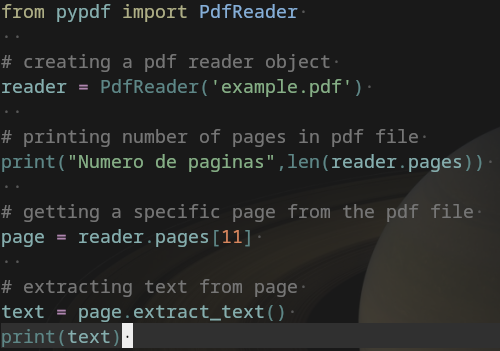
\includegraphics[scale=0.5]{pypdf_1}
		\caption{Uso de la librería PyPDF}
		\small
		%Fuente: Autor
	\end{figure}
		\begin{figure}[H]
		\centering
		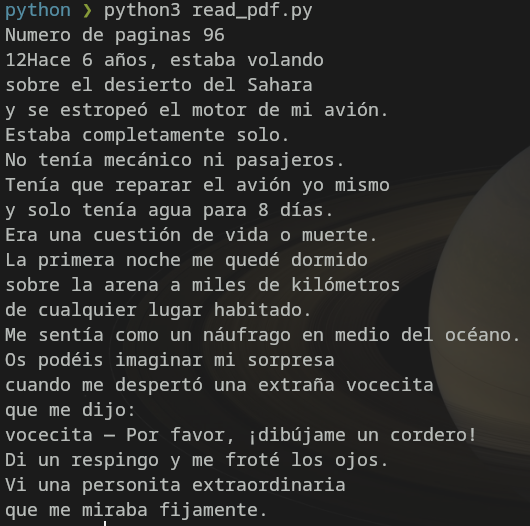
\includegraphics[scale=0.5]{pypdf_2}
		\caption{Uso de la librería PyPDF}
		\small
		%Fuente: Autor
	\end{figure}
	%\begin{itemize}
		%\item GTP-1
		%\item GTP-2
		%\item GTP-3
		%\item GTP-4
		%\item Megatron-LM
		%\item PaLM
		%\item LaMDA
		%\item GPT-Neo
		%\item GPT-J
	%	\item BERT
%		\item RoBERTa
		%\item T5
	%	\item DistilBERT
%	\end{itemize}

\begin{table}[h!]
	\centering
	\begin{tabular}{|l|l|l|l|}
		\hline
		\textbf{Modelo} & \textbf{Capacidad de Tokenización (Límite de Contexto)} & \textbf{Tipo}       & \textbf{Número de Parámetros} \\ \hline
		GPT-1           & 512 tokens                                              & Pago                & 117M                         \\ \hline
		GPT-2           & 1024 tokens                                             & Código libre        & 1.5B                         \\ \hline
		GPT-3           & 2048 tokens                                             & Pago                & 175B                         \\ \hline
		GPT-4           & Hasta 8192 tokens o más, dependiendo de la configuración & Pago                & 175B+                        \\ \hline
		Megatron-LM     & 2048 tokens                                             & Código libre        & 8.3B                         \\ \hline
		PaLM            & 2048 tokens                                             & Pago                & 540B                         \\ \hline
		LaMDA           & Hasta 2048 tokens                                       & Pago                & 137B                         \\ \hline
		GPT-Neo         & 2048 tokens                                             & Código libre        &1.3B y 2.7B                         \\ \hline
		GPT-J           & 2048 tokens                                             & Código libre        & 6B                           \\ \hline
		BERT            & 512 tokens                                              & Código libre        & 110M                         \\ \hline
		RoBERTa         & 512 tokens                                              & Código libre        & 355M                         \\ \hline
		T5              & 512 tokens                                              & Código libre        & 11B                          \\ \hline
		DistilBERT      & 512 tokens                                              & Código libre        & 66M                          \\ \hline
	\end{tabular}
	\caption{Capacidad de Tokenización, Tipo y Número de Parámetros de LLMs identificados}
	\label{tab:tokenization}
\end{table}
	\section{LLMs seleccionados}
	\subsection{GPT-Neo}
	"Hace 6 años, estaba volando sobre el desierto del Sahara y se estropeó el motor de mi avión. Estaba completamente solo"\ref{table:1}.
	\begin{figure}[H]
	\centering
	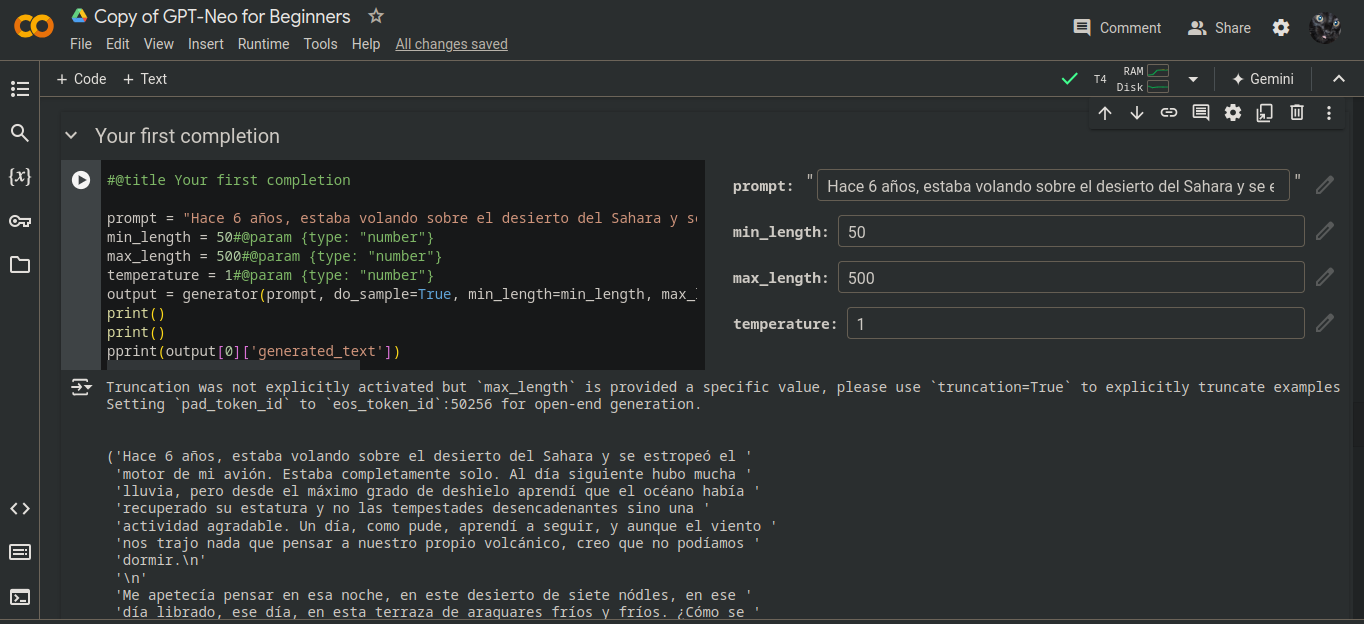
\includegraphics[scale=0.5]{gptneo_1}
	\caption{Ejemplo GPT-Neo}
	\small
	\label{table:1}
	%Fuente: Autor
\end{figure}
	\begin{figure}[H]
	\centering
	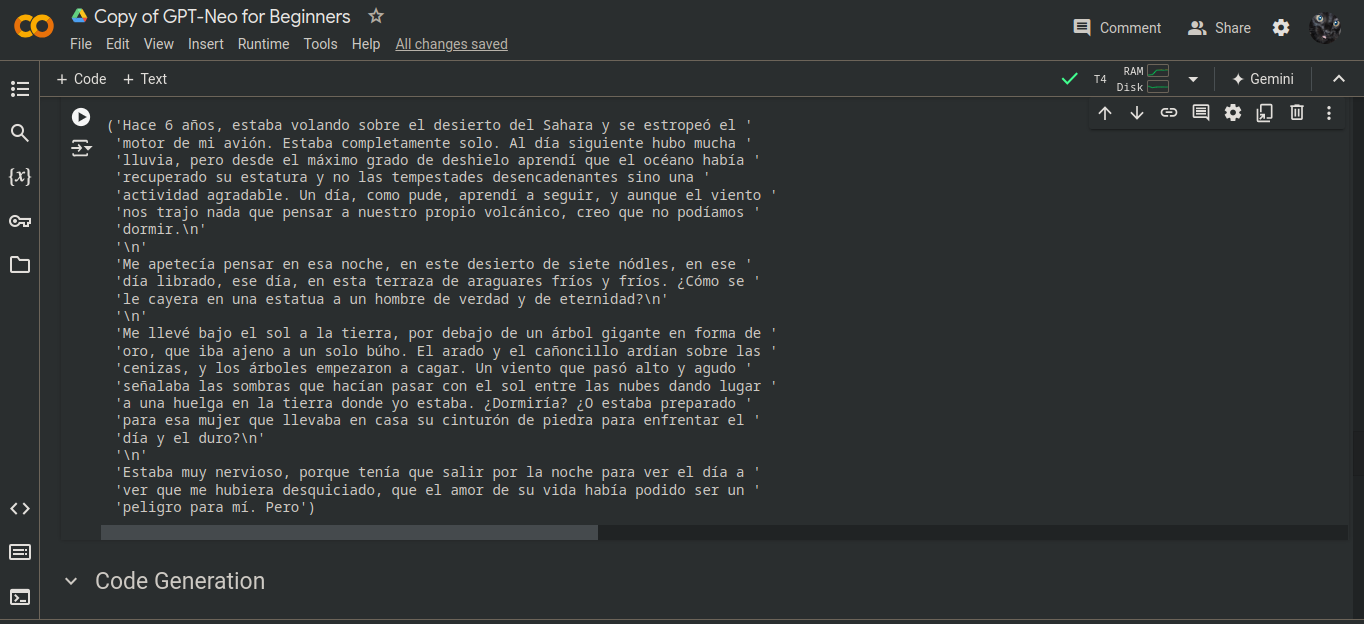
\includegraphics[scale=0.5]{gptneo_2}
	\caption{Ejemplo GPT-Neo}
	\small
	%Fuente: Autor
\end{figure}
	\subsection{T5}
	\begin{figure}[H]
		\centering
		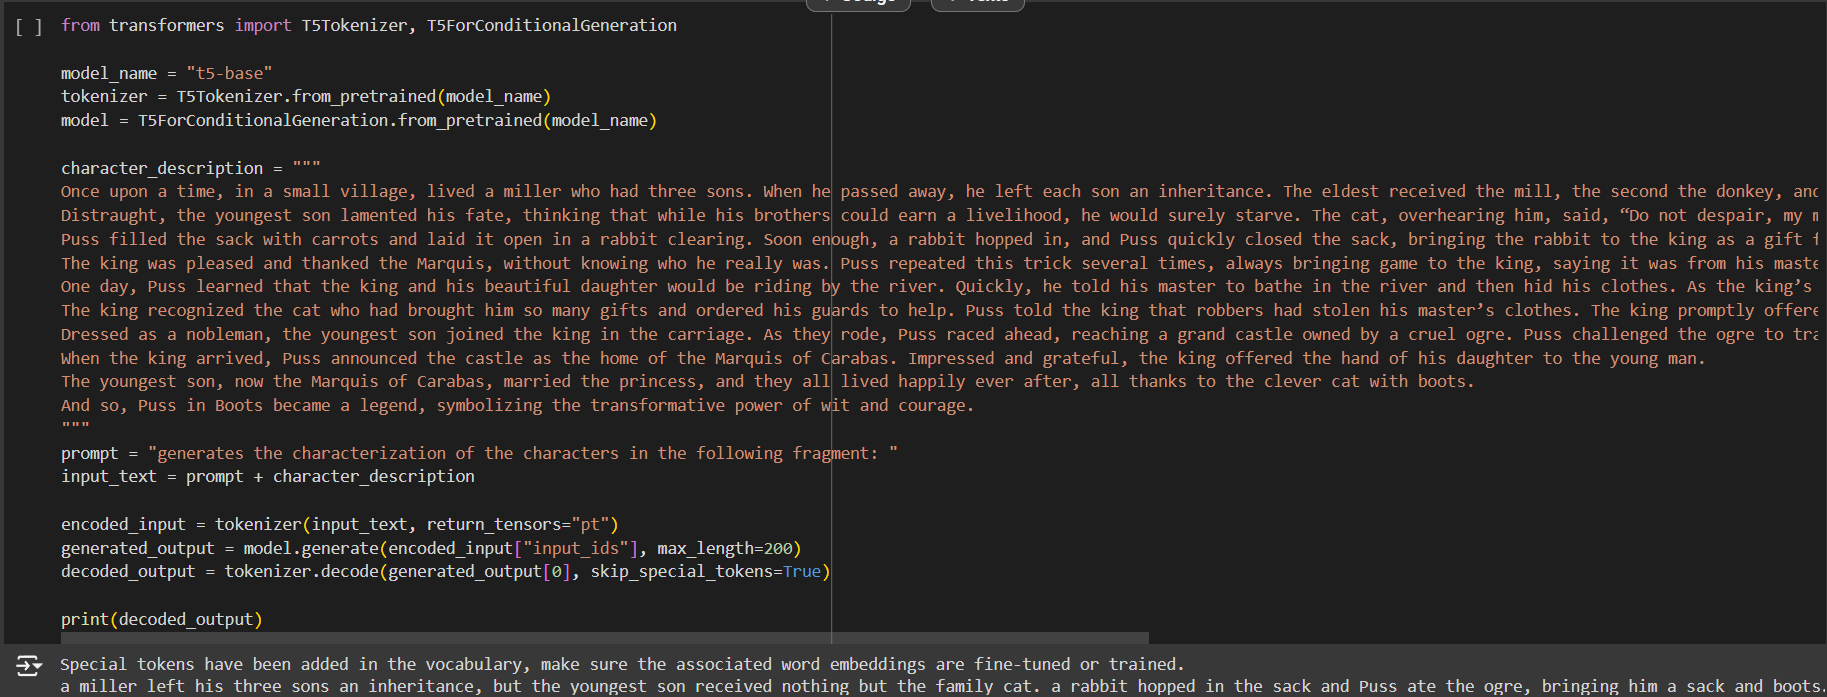
\includegraphics[scale=0.5]{t5test1}
		\caption{Ejemplo caracterizacion de personajes T5.}
		\small
%Fuente: Autor
	\end{figure}
	
	\begin{figure}[H]
		\centering
		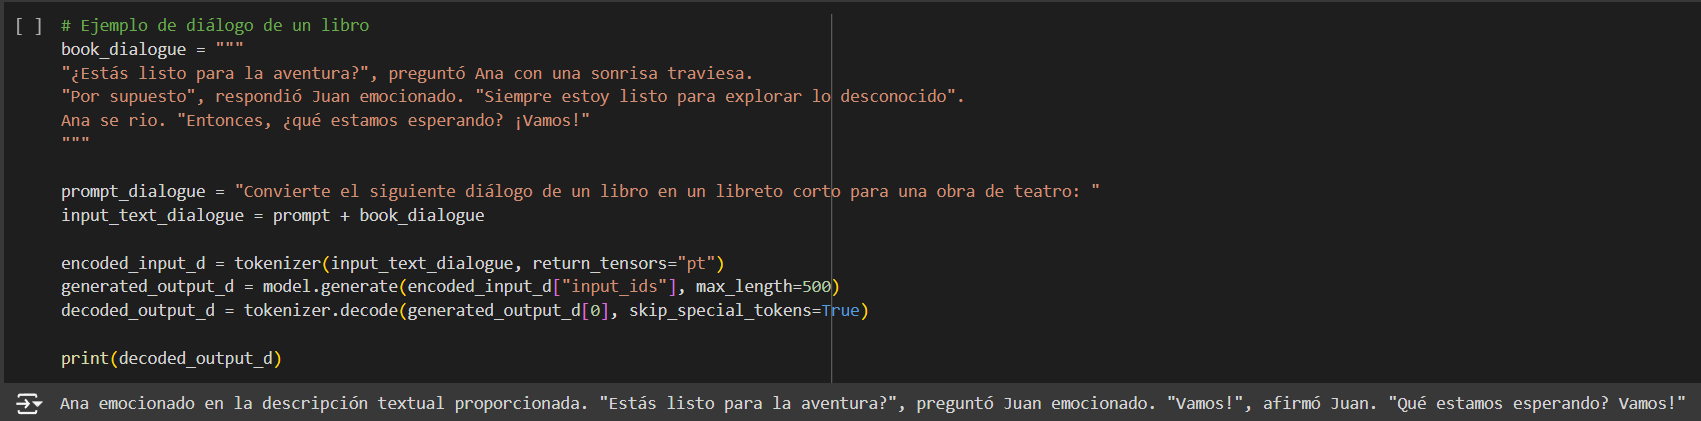
\includegraphics[scale=0.5]{t5test2}
		\caption{Ejemplo generación libreto T5.}
		\small
		%Fuente: Autor
	\end{figure}
	
	
	\subsection{GPT-4}
	\begin{figure}[H]
		\centering
		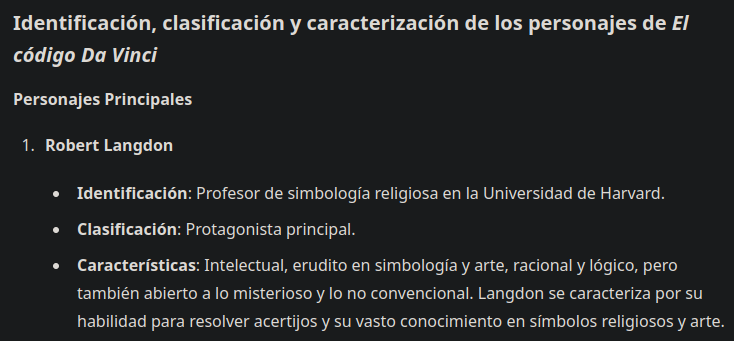
\includegraphics[scale=0.5]{gpt4_1}
		\caption{Identificación, caracterización y clasificación de personajes: El código Da Vinci}
		\small
		%Fuente: Autor
	\end{figure}
	\begin{figure}[H]
		\centering
		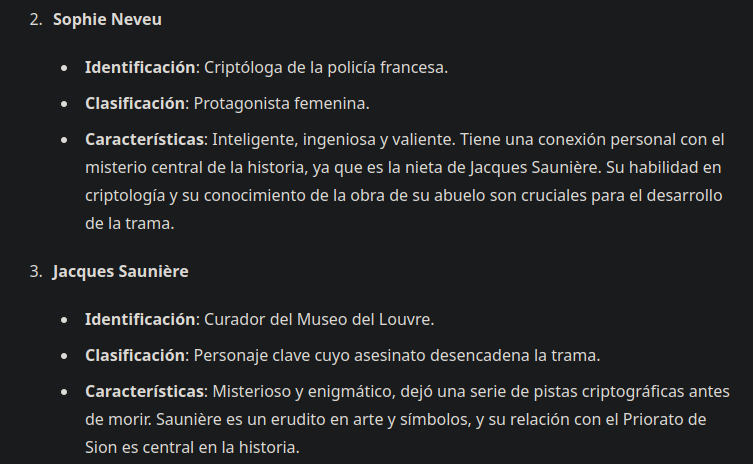
\includegraphics[scale=0.5]{gpt4_2}
		\caption{Identificación, caracterización y clasificación de personajes: El código Da Vinci}
		\small
		%Fuente: Autor
	\end{figure}
	\begin{figure}[H]
		\centering
		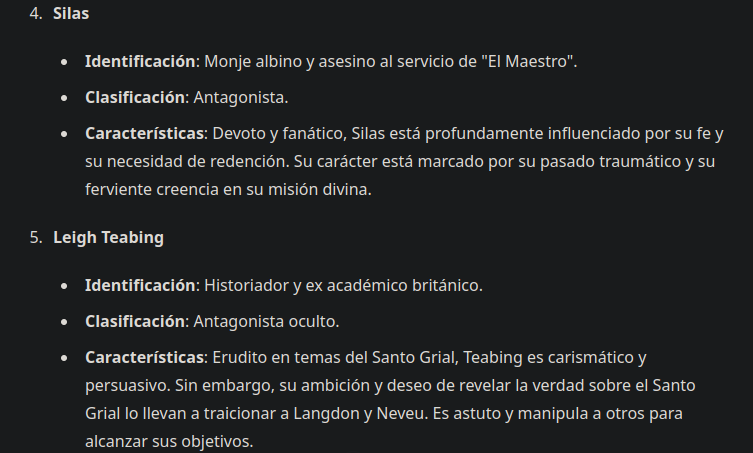
\includegraphics[scale=0.5]{gpt4_3}
		\caption{Identificación, caracterización y clasificación de personajes: El código Da Vinci}
		\small
		%Fuente: Autor
	\end{figure}
	\begin{figure}[H]
		\centering
		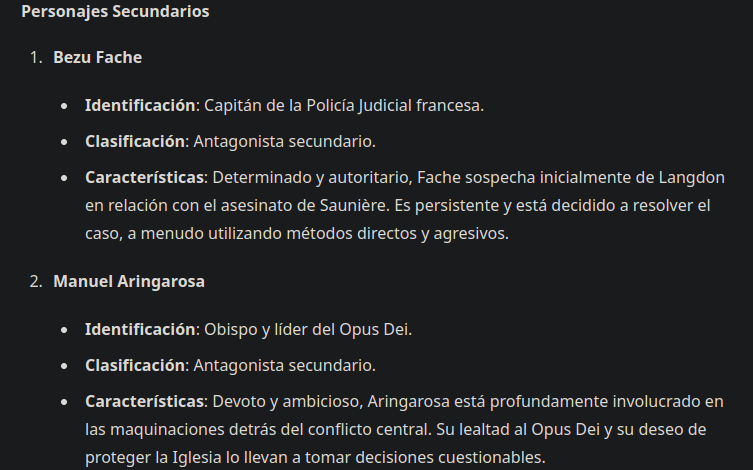
\includegraphics[scale=0.5]{gpt4_4}
		\caption{Identificación, caracterización y clasificación de personajes: El código Da Vinci}
		\small
		%Fuente: Autor
	\end{figure}
	\section{Fuentes de datos seleccionados}
	\begin{itemize}
		\item Libros de cuentos y relatos cortos: Los libros de cuentos y relatos cortos son una fuente viable de fragmentos narrativos concisos, que podrían servir como base para desarrollar cortometrajes. Algunos ejemplos son los cuentos de Edgar Allan Poe, Anton Chéjov, Jorge Luis Borges, entre otros.
		\item Antologías de historias cortas: Las antologías recopilan historias cortas de diversos autores y géneros, lo que te brindaría una amplia variedad de estilos y temáticas para trabajar.
		\item Novelas cortas: Las novelas cortas, también conocidas como "novellas", son obras narrativas más extensas que un cuento, pero más breves que una novela completa. Podrías extraer fragmentos o capítulos completos de estas obras.
		\item Obras de teatro de un acto: Las obras de teatro de un acto, al ser más cortas y condensadas, son una excelente fuente de diálogos y tramas compactas que podrían adaptarse fácilmente a cortometrajes.
		\item Repositorios de guiones y libretos: Existen repositorios en línea que compilan guiones y libretos de películas, series de televisión y obras de teatro. Aunque no son fragmentos literarios, podrían ser útiles para aprender sobre la estructura y el formato de los libretos.
		\item Sitios web y plataformas de escritura creativa: Algunas plataformas en línea, como Wattpad, Inkitt o WritingPrompts, albergan historias cortas, relatos y escritos creativos de autores emergentes. Estos podrían ser una fuente interesante de material.
	\end{itemize}
	\section{Hallazgos}
	Existen diferentes opciones de LLMs, particularmente de código y uso libre. Pero es evidente que las herramientas que mejor rendimiento y calidad de salida tienen son las que tienen costo por su uso, específicamente GPT-4 realiza exitosamente la tarea de identificar, caracterizar y clasificar personajes.
	Dentro de la capa gratuita de GPT-4 podemos obtener datos de la identificación, caracterización y clasificación de personajes para el LLM seleccionado.
	\section{Conclusión}
	Partiendo de los aspectos generales de los LLMs identificados,  descartamos los que tuvieran asociado un costo para su uso. Además se identificó y seleccionó el LLMs que provee una mayor capacidad de tokenización, siendo en este caso GPT-Neo.
	
	\section{Bibliografía}
		\renewcommand\refname{Referencias}
	\bibliographystyle{apalike}
	\bibliography{./references.bib}
	


\end{document}